\chapter{Tecnoloxías de contedorización}
\minitoc
\clearpage

\section{Introdución das tecnoloxías}

Neste capítulo realizarase unha breve introdución e comparativa das tecnoloxías de contedorización a empregar ao longo deste traballo. Un breve resumo de achegamento pode ser consultado na táboa \ref{comparativaTecnoloxiasContedorizacion}.

\begin{table}[H]
\centering
\caption{Comparativa das tecnoloxías de contedorización}
\label{comparativaTecnoloxiasContedorizacion}
\resizebox{\textwidth}{!}{%
\begin{tabular}{|l|c|c|c|}
\hline
                        & \textbf{Singularity} & \textbf{Docker} & \textbf{UDocker} \\ \hline
Modelo de privilexios & SUID & Demo Root & Sen privilexios \\ \hline
Non precisas configuracións adicionais de rede & \color[HTML]{006600}{\cmark} & \textcolor{red}{\xmark} & \textcolor{red}{\xmark} \\ \hline
Soporte nativo para GPU & \color[HTML]{006600}{\cmark} & \textcolor{red}{\xmark}* & \color[HTML]{006600}{\cmark} \\ \hline
Soporte nativo para InfiniBand & \color[HTML]{006600}{\cmark} & \color[HTML]{006600}{\cmark} & \color[HTML]{006600}{\cmark} \\ \hline
Deseñado para uso científico & \color[HTML]{006600}{\cmark} & \textcolor{red}{\xmark} & \textcolor{red}{\xmark} \\ \hline
% &  &  &  \\ \hline
\end{tabular}
}
*Precisa configuracións.
\end{table}

Indicar que tanto Udocker como Singularity xa están instalados e configurados para a súa emprega a todos os usuario dende o sistema de módulos do \gls{FT2}.

\section{Docker}

\subsection{Funcionamento}

Correr contedores baixo a tecnoloxía de Docker implica correr o demo Docker. Dito demo precisa actualmente de privilexios de superusuario, e unha serie de detalles deben ser tidos en conta. Por exemplo, só debemos deixar que usuarios autorizados fagan uso do demo de Docker, xa que se un ataque contra este demo tivera éxito, o atacante posuiría permisos de superusuario no sistema. É dicir, só usuarios autorizados deberían ser quen de despregar contedores no sistema.\\

Explicado dun xeito sinxelo, Docker basea o seu modelo de privilexios nun demo, que debe correr con privilexios de superusuario, e que pode ser contactado polos usuarios a través de clientes que se comunicarán con dito demo grazas ao \textit{endpoint} \gls{API} \gls{REST} que posúe. Este esquema pode ser observado na figura \ref{dockerStructure}. No referente ao despregamento, o proceso e a utilización deste demo quedan recollidos na figura \ref{dockerStructure2}.\\

\begin{figure}
\centerline{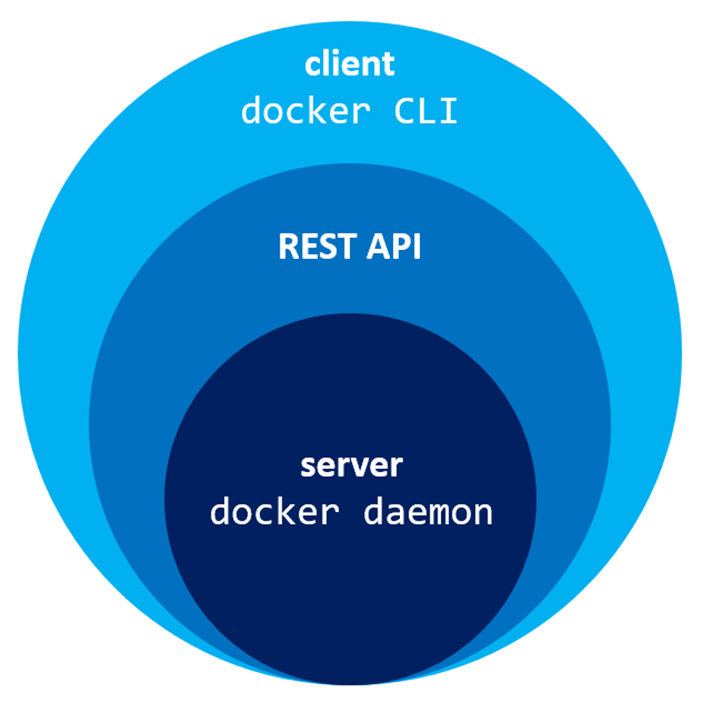
\includegraphics[width=10cm]{figuras/dockerStructure}}
\caption{Esquema de funcionamento de Docker}
\medskip
\small
\centerline{Fonte: \url{https://www.aquasec.com/wiki/display/containers/Docker+Containers}}
\label{dockerStructure}
\end{figure}

\begin{figure}
\centerline{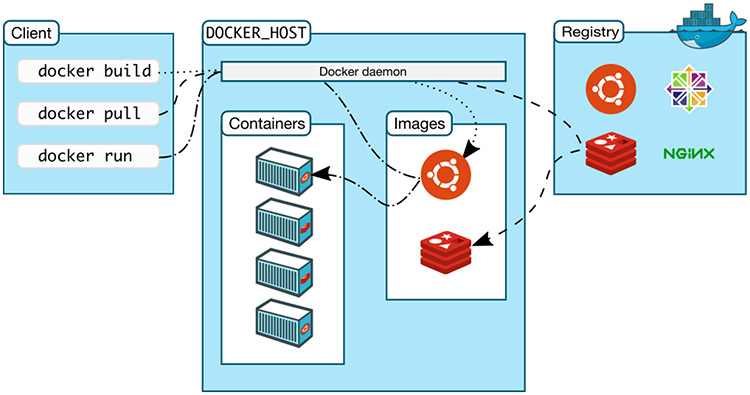
\includegraphics[width=15cm]{figuras/dockerStructure2}}
\caption{Modelo de despregamento de contedores en Docker}
\medskip
\small
\centerline{Fonte: \url{https://www.aquasec.com/wiki/display/containers/Docker+Containers}}
\label{dockerStructure2}
\end{figure}

\subsection{Seguridade}

Isto ten importantes implicacións de seguridade: exemplificando, se lanzamos Docker dende un servidor web para aprovisionar contedores a través dunha \gls{API}, deberiamos ser máis coidadosos do habitual coa comprobación de parámetros e outras medidas de seguridade para asegurar que un usuario malintencionado non poida pasar parámetros elaborados, facendo que o demo de Docker cree contedores arbitrarios.\\

Motivado por esta fenda de seguridade, o \textit{endpoint} da \gls{API} \gls{REST} de Docker trocou dun simple \textit{socket} \gls{TCP} a un \textit{socket} UNIX na súa versión 0.5.2, xa que o primeiro é considerado moito máis propenso a ataques \textit{cross-site}, se o demo se executa directamente na máquina anfitrioa e non está protexido por unha capa extra de virtualización mediante \gls{MV}s.

\section{Singularity}

\subsection{Funcionamento}

O primeiro que debemos comprender á hora de tratar con contedores Singularity é que esta tecnoloxía non parte da base de usuarios autorizados executando contedores autorizados, como moitas das tecnoloxías de contedorización existentes. Baixo ese enfoque, a tecnoloxía de contedorización debe ser controlada por un superusuario ou un usuario que fose autorizado para executar con permisos de tal. Alterando este punto de vista, o enfoque de Singularity parte da premisa de tratarse dunha tecnoloxía especializada para infraestruturas \gls{HPC}, onde existen moitos usuarios, pero case ningún deles é considerado fiábel, o que significa que é preciso abordar un paradigma distinto no que se deben soportar contedores non fiábel executados por usuarios non fiábeis. \cite{SingularitySecurity}\\

Para acadar este funcionamento, Singularity fai uso das seguintes ferramentas:

\begin{itemize}
    \item \textbf{SetUID:} este é o modelo predeterminado, posto que oferta a maior flexibilidade, mais tamén é o que máis riscos presenta dende a perspectiva da seguridade. Simplificando o seu funcionamento, un programa co SetUID activado por \textit{root}, poderá ser executado por outro usuario cos mesmos privilexios que \textit{root}. Por esta razón, os programas co SetUID activado son obxectivos habituais para os atacantes. Tendo isto en mente, Singularity foi desenvolvido atendendo á simplicidade e á lexibilidade, e só son outorgados privilexios de superusuario cando son estritamente precisos, quedando desactivados inmediatamente despois. Concretamente, as tarefas que precisan desta escalada de privilexios controlada son:
    \begin{itemize}
        \item Montaxe da imaxe no contedor Singularity.
        \item Creación dos espazos de nomes necesarios, coa axuda do \textit{kernel}.
        \item Compartición de directorios entre o contedor e a máquina anfitrioa, se así foi requirido.
    \end{itemize}
    Estes compoñentes co SetUID activado poden ser activados ou desactivados a pracer, tanto no momento da instalación como despois. Non obstante, perderemos as capacidades que estes outorgan.
    \item \textbf{Espazos de nomes:} Singularity admite a emprega de espazos de nomes de usuario de xeito nativo e poden executarse completamente sen privilexios dende a versión 2.2, mais cunhas funcionalidades moi limitadas. Por exemplo, só será posíbel empregar contedores baseados nun directorio. Ademais, posto que os espazos de nomes non son compatíbeis con todos os \textit{kernels} a súa empregabilidade pode variar.
\end{itemize}

\subsection{Fluxo de traballo}

O fluxo de funcionamento de Singularity normalmente implica que o usuario desenvolva nun dispositivo local ou nunha máquina virtual, no cal teña permisos de superusuario, e unha vez finalizado o desenvolvemento mova o contedor ao entorno de produción. En dito entorno non terá permisos de superusuario e non poderá facer cambios que requiran dos mesmos dentro do contedor, mais a solución é tan simple como volver ao entorno de desenvolvemento e facer os cambios pertinentes. Este modelo queda recollido na figura \ref{singularityWorkflow} dun xeito xeral, e na figura \ref{singularity-workflow} para o caso concreto do \gls{CESGA} sobre o \gls{FT2}.

\begin{figure}
\centerline{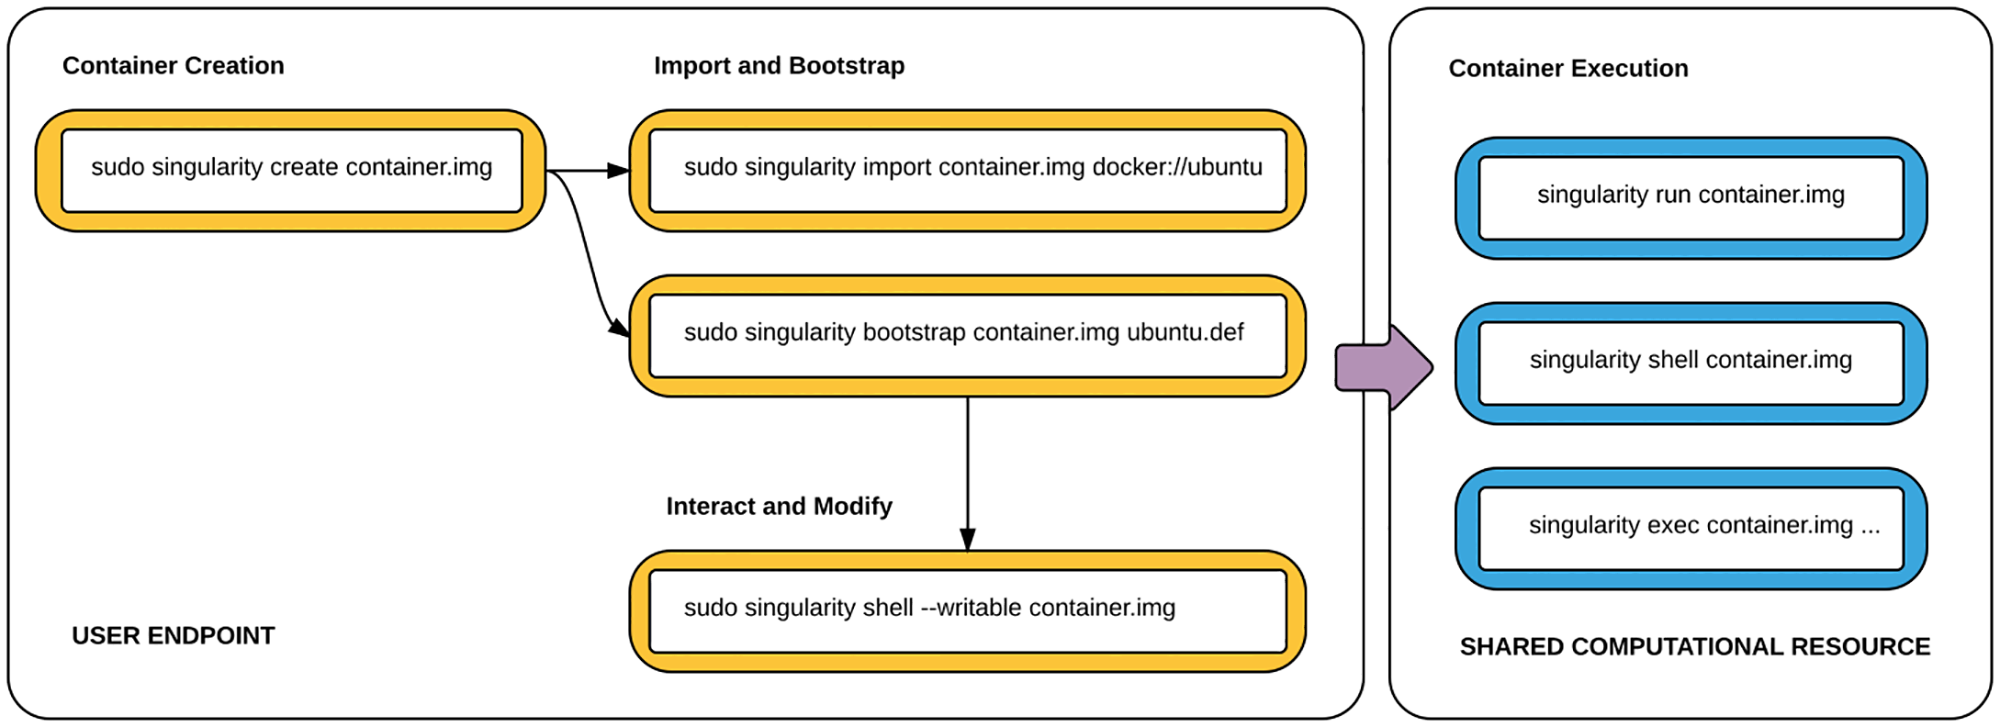
\includegraphics[width=15cm]{figuras/singularityWorkflow}}
\caption{Modelo de despregamento de contedores en Singularity}
\medskip
\small
\centerline{Fonte: \url{https://singularity.lbl.gov/}}
\label{singularityWorkflow}
\end{figure}

\begin{figure}
\centerline{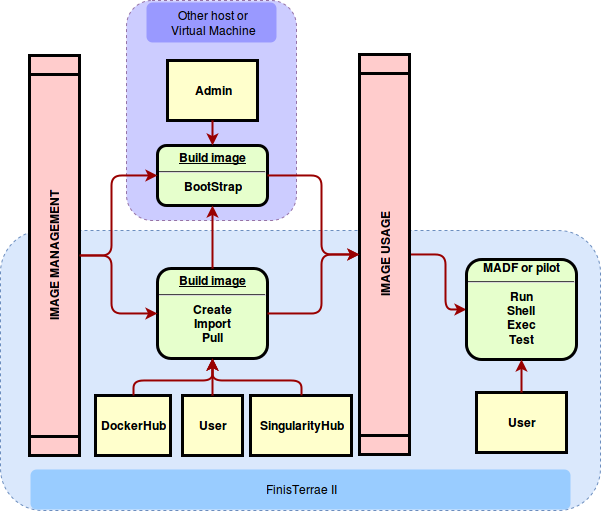
\includegraphics[width=15cm]{figuras/singularity-workflow.png}}
\caption{Modelo de despregamento de contedores en Singularity sobre \gls{FT2}}
\medskip
\small
\centerline{Fonte: \cite{MSO4SC}}
\label{singularity-workflow}
\end{figure}

\subsection{Seguridade}

O modelo de funcionamento de Singularity fai que se trate dunha ferramenta coa que dificilmente se poida abordar un ataque de escalada de privilexios, algo moi importante en entornos multiusuario. Isto é así porque o usuario a empregar unha vez lanzadas as execucións dos contedores é o mesmo usuario que está fóra do contedor. Se un usuario desexa ser superusuario dentro do contedor, primeiramente debe ser superusuario fóra do contedor.

\subsection{Compatibilidade con contedores Docker}

Posto que Docker estase a converter nun estándar na industria, resulta interesante poder ler e traballar con este tipo de contedores e aproveitar gran cantidade de traballo xa realizado. Así, Singularity soporta o tratamento de contedores Docker, sen ter que ter instalada dita tecnoloxía. Isto faise  mediante a emprega da \gls{API} do Docker Registry, unha interface \gls{REST} que da acceso aos manifestos das imaxes, cada un dous cales contén información sobre as capas das imaxes. Cada capa non é máis que un conxunto comprimido de carpetas e arquivos que poden ser extraídos directamente nunha imaxe Singularity. \cite{singularityScientificContainers}

\section{Udocker}
\label{introUdocker}

\subsection{Funcionamento}

Udocker é unha ferramenta que permite executar contedores simples de Docker nun espazo de usuario sen requirir de privilexios de superusuario, permitindo así a descarga e a execución de contedores Docker por usuarios non privilexiados en entornos Linux onde Docker non está dispoñíbel.\\

Pode ser empregado sen ningún tipo de privilexios no despregamento do servizo por parte do administrador do sistema, pudendo ser descargado e executado enteiramente polo usuario final.\\

Trátase dunha ferramenta sinxela escrita en Python, cun conxunto mínimo de dependencias que permiten que poida ser executado nun gran rango de entornos Linux, sen precisar tan sequera ter Docker instalado. O seu funcionamento baséase na emprega dun entorno tipo ``\textit{chroot}'', pero de xeito imitado, para non requirir privilexios en dito entorno. Para iso fai uso dunha serie de ferramentas e librarías coma poden ser:

\begin{itemize}
    \item PRoot
    \item Fakechroot
    \item runC
    \item Singularity
\end{itemize}

Este xeito de funcionar outorga unha serie de vantaxes. Por exemplo, o usuario final non terá que aprender unha nova ferramenta, pois de cara el compórtase exactamente como Docker (mesmos contedores, mesmos comandos, etc.). O usuario tampouco requirirá da axuda do administrador para despregar contedores nun equipo compartido, xa que non son precisos privilexios para a súa execución nin para a súa instalación; de feito, ao estar escrito en Python, nin tan sequera é preciso realizar o proceso de compilación, simplemente lanzar o script e executar. Destacar finalmente que foi testado sobre procesamento paralelo con aplicacións \gls{MPI} e \gls{GPGPU}. \cite{UdockerDoc}

\subsection{Limitacións}

Ao non existiren privilexios de superusuario involucrados, calquera operación que realmente precise ditos privilexios non será realizábel. Por exemplo, con Udocker é imposíbel realizar operacións como as seguintes:

\begin{itemize}
    \item Acceder a ficheiros e dispositivos protexidos pola máquina anfitrioa.
    \item Escoitar en portos TCP/IP privilexiados (rango embaixo do 1024).
    \item Montar sistemas de ficheiros.
    \item Emprega do comando \textit{su}.
    \item Cambio da hora do sistema.
    \item Operacións de rede complexas, tales como:
    \begin{itemize}
        \item Cambiar as táboas de enrutamento.
        \item Modificar regras nunha devasa.
        \item Tratamento con interfaces de rede.
    \end{itemize}
\end{itemize}

No caso de precisar realizar operacións como as anteriores, Udocker non é a tecnoloxía de contedorización adecuada e debemos optar por solucións alternativas. \cite{UdockerDoc}

\subsection{Seguridade}

O modelo de Udocker convérteo nunha solución relativamente segura, no sentido de que un atacante xamais poderá realizar un ataque de escalada de privilexios, ao non existir en ningún momento estes privilexios.\\

Non obstante, debido ás limitacións explicadas na sección anterior, Udocker non ofrece características avanzadas de illamento como poden ter outras tecnoloxías. Polo tanto, se o contido dos contedores non é fiábel, non debería ser executado baixo Udocker, xa que estes se executarán dentro do propio entorno do usuario. Os datos estarán suxeitos ás mesmas proteccións do sistemas que os outros arquivos propiedade do usuario.\\

Polo tanto, debido a esta falta de illamento, Udocker nunca debe ser executado por usuarios con privilexios.\\
